\chapter{Resultats et evaluation}
\label{chap:resultats-evaluation}

\section{Jeu de documents traite}

Le jeu de test utilise pendant le stage est stocke dans un dossier dedie compatible avec OneDrive. Il contient 35 documents: 17 factures et 18 devis. Les formats PDF, JPG et PNG ont permis de tester a la fois des documents numeriques et des images scannees.

Les resultats montrent que le pipeline est capable d'extraire les informations principales, de les stocker dans Postgres, de generer des embeddings en dimension 1536 et de retrouver les documents pertinents par recherche hybride.

\section{Exemples d'interrogation de l'agent}

L'agent RAG permet de poser des questions en langage naturel sur les documents traites. Les tests incluent des questions simples et des requetes avec filtres, par exemple sur un fournisseur ou une agregation.

\begin{figure}[H]
\center
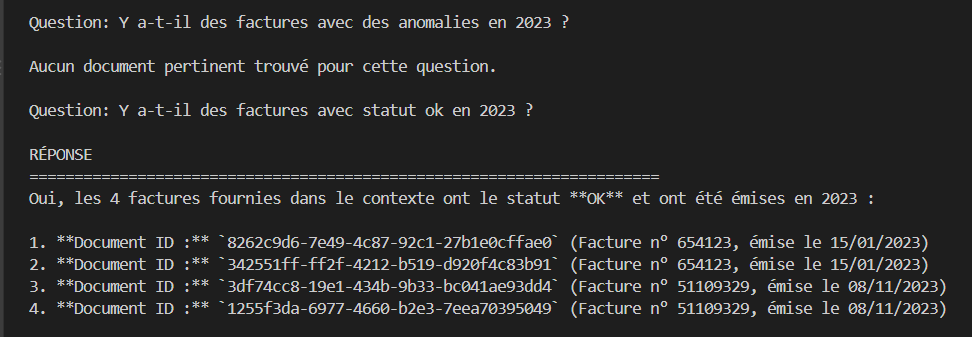
\includegraphics[width=0.9\textwidth]{images/test_simple.png}
\caption[Test simple de l'agent]{Exemple de question simple adressee a l'agent RAG.}
\label{fig:test-simple}
\end{figure}

\begin{figure}[H]
\center
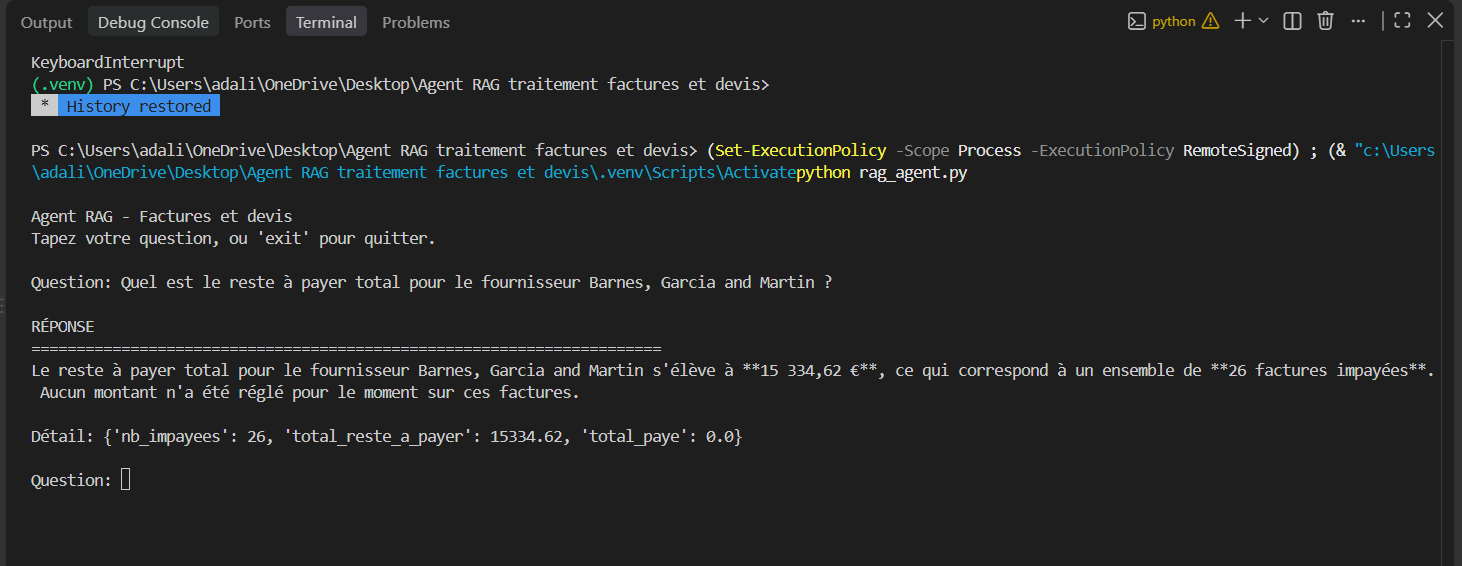
\includegraphics[width=0.9\textwidth]{images/filtre_fournisseur__aggregation.png}
\caption[Filtre fournisseur et agregation]{Exemple de requete combinant filtre fournisseur et logique d'agregation.}
\label{fig:filtre-fournisseur}
\end{figure}

\section{Rapports generes}

Le module de reporting produit des rapports Excel et HTML a partir des donnees Postgres. Les graphiques utilisent un regroupement \textit{Top 8 + Autres} afin de garder une visualisation lisible lorsque le nombre de fournisseurs ou categories augmente.

\begin{figure}[H]
\center
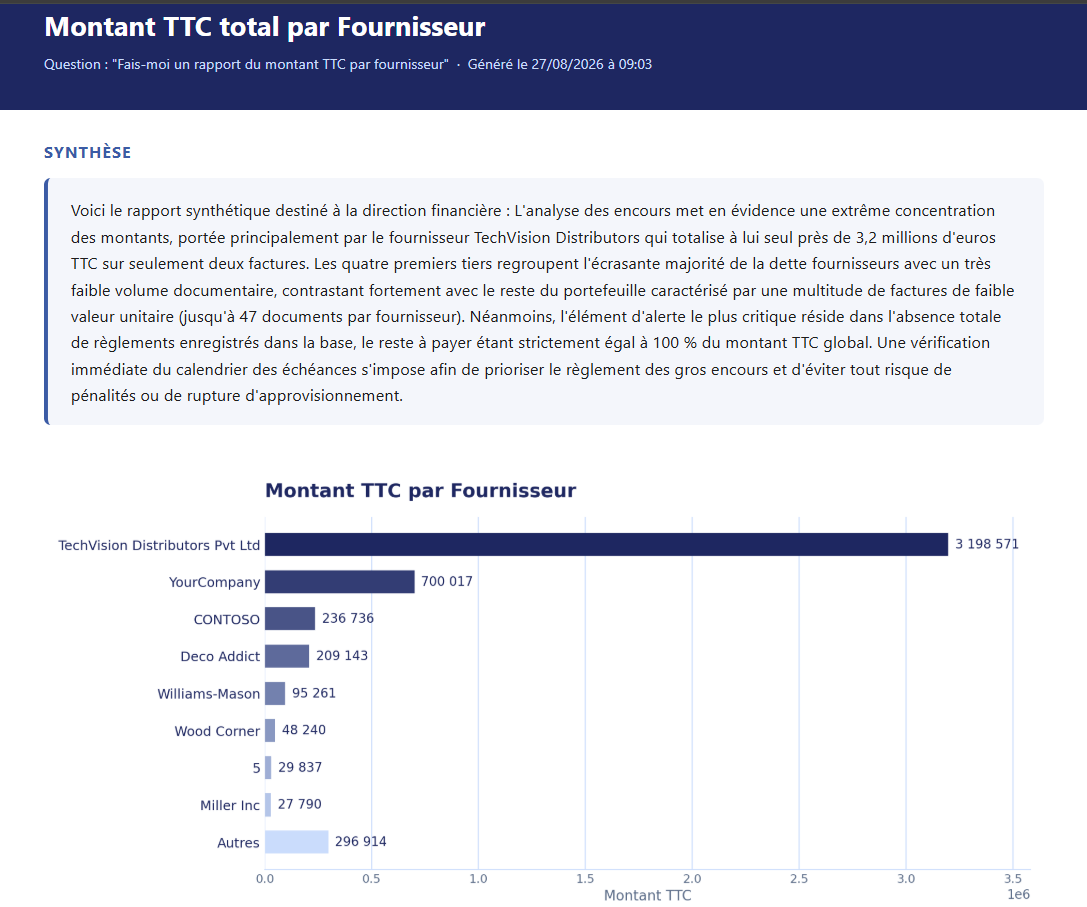
\includegraphics[width=0.9\textwidth]{images/rapport1_1.png}
\caption[Rapport genere premier exemple]{Premier exemple de rapport genere automatiquement, partie 1.}
\label{fig:rapport1-1}
\end{figure}

\begin{figure}[H]
\center
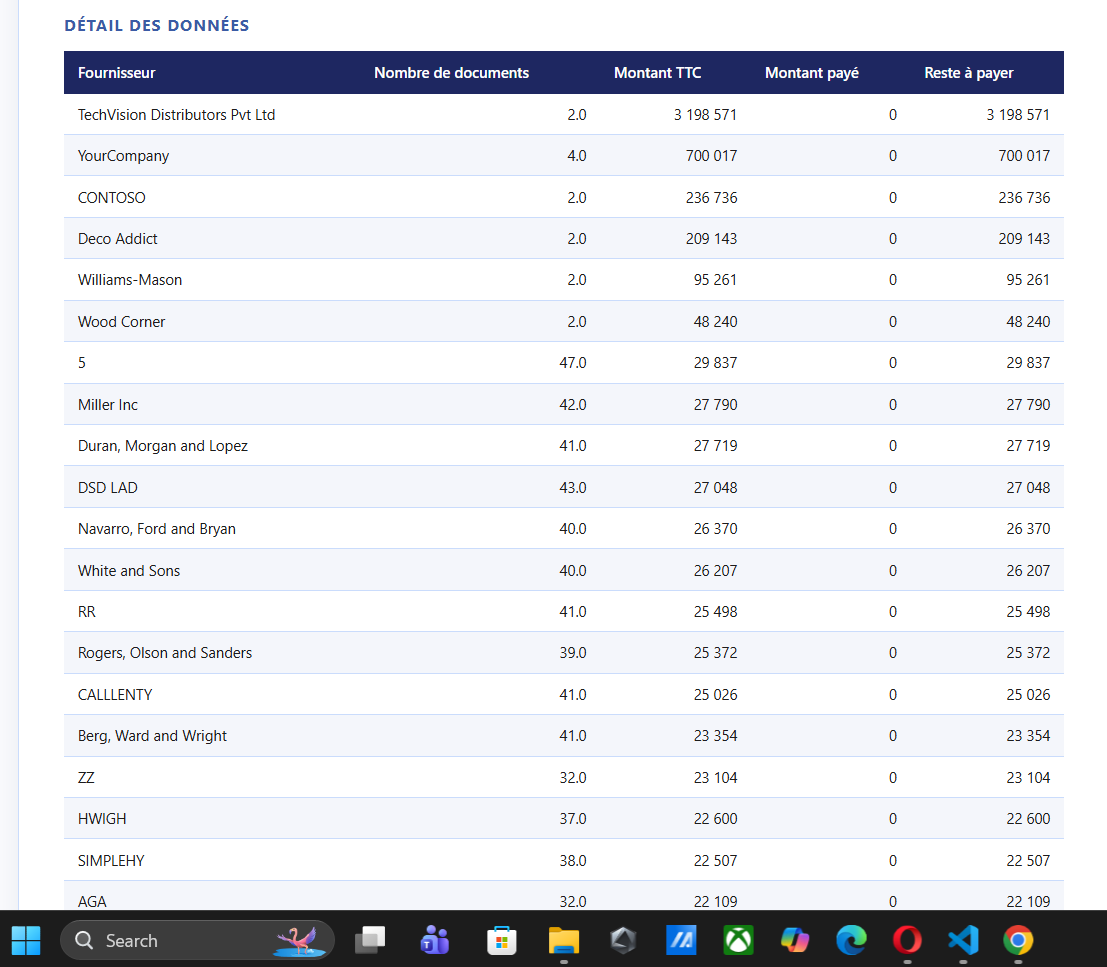
\includegraphics[width=0.9\textwidth]{images/rapport1_2.png}
\caption[Rapport genere premier exemple suite]{Premier exemple de rapport genere automatiquement, partie 2.}
\label{fig:rapport1-2}
\end{figure}

\begin{figure}[H]
\center
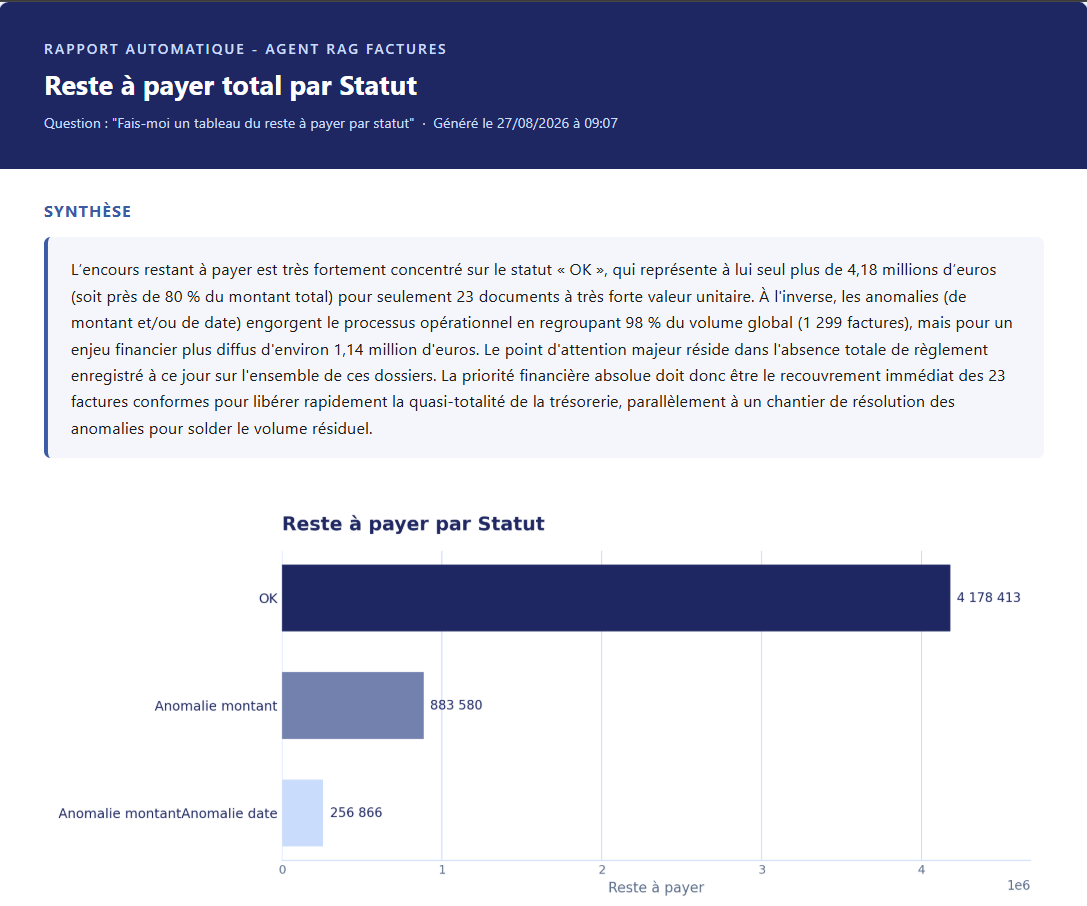
\includegraphics[width=0.9\textwidth]{images/rapport2_1.png}
\caption[Rapport genere deuxieme exemple]{Deuxieme exemple de rapport genere automatiquement, partie 1.}
\label{fig:rapport2-1}
\end{figure}

\begin{figure}[H]
\center
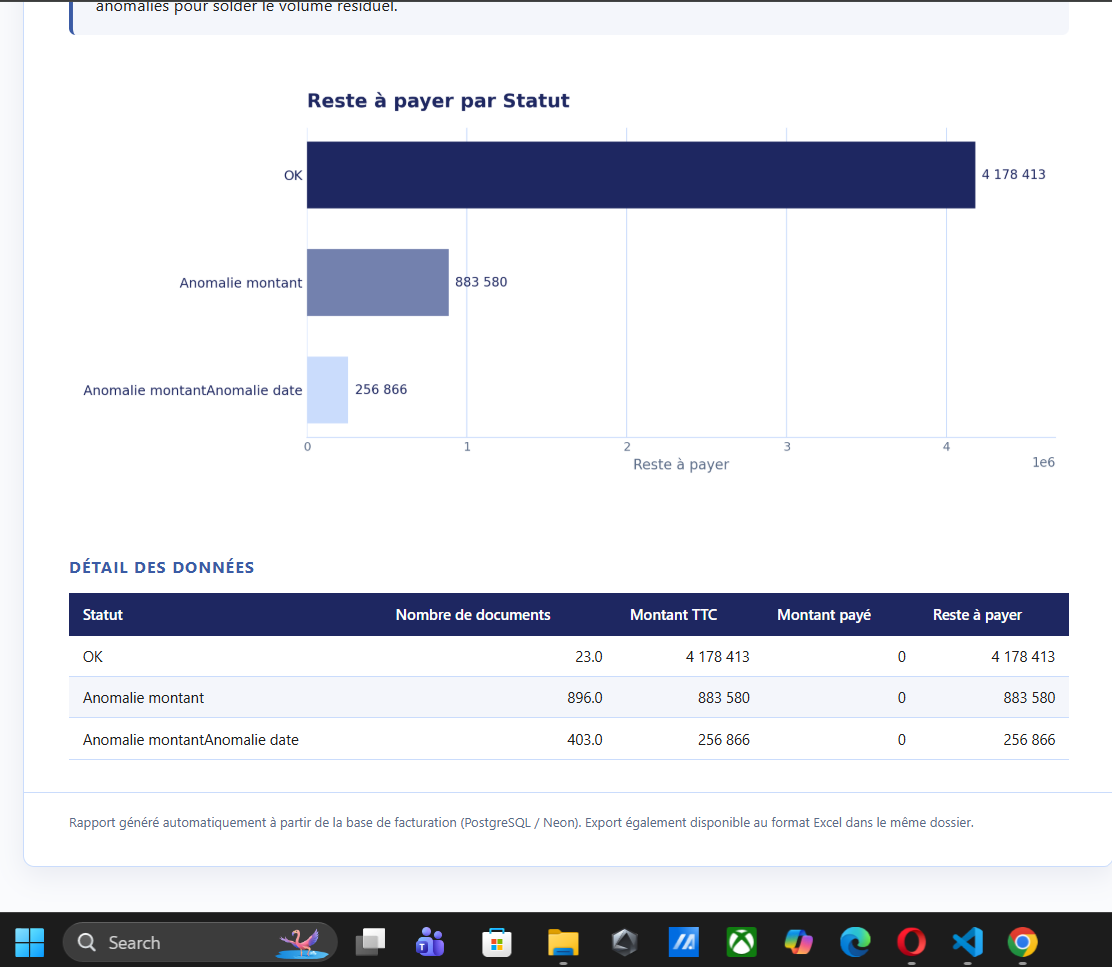
\includegraphics[width=0.9\textwidth]{images/rapport2_2.png}
\caption[Rapport genere deuxieme exemple suite]{Deuxieme exemple de rapport genere automatiquement, partie 2.}
\label{fig:rapport2-2}
\end{figure}

\begin{figure}[H]
\center
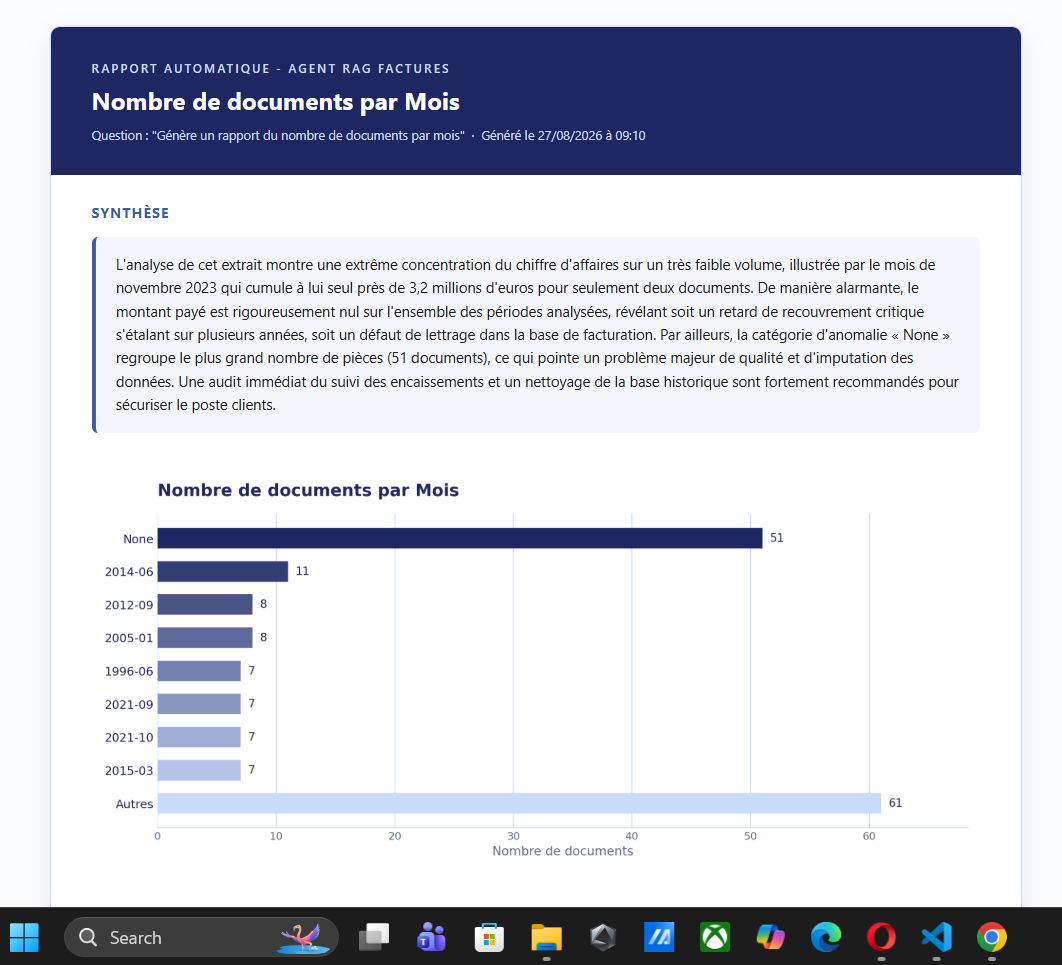
\includegraphics[width=0.9\textwidth]{images/rapport3_1.png}
\caption[Rapport genere troisieme exemple]{Troisieme exemple de rapport genere automatiquement, partie 1.}
\label{fig:rapport3-1}
\end{figure}

\begin{figure}[H]
\center
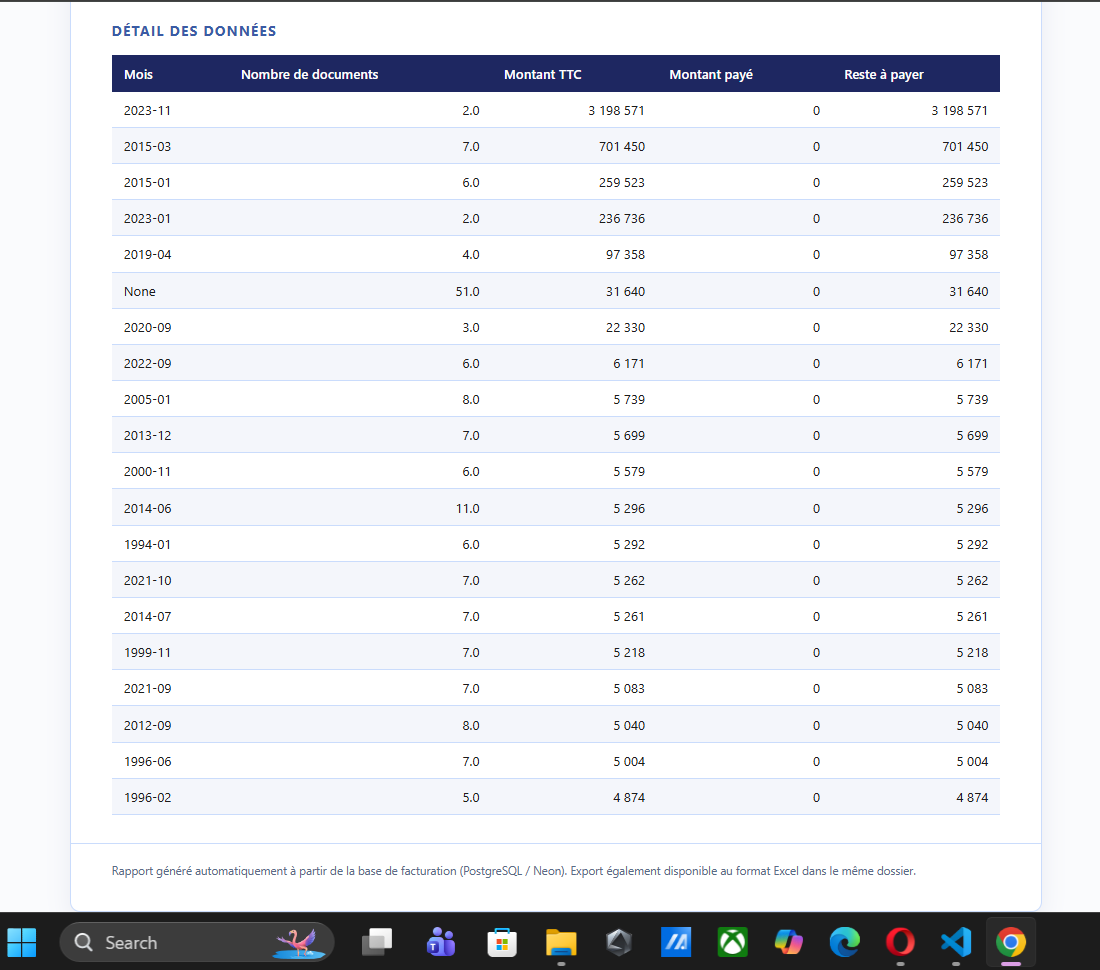
\includegraphics[width=0.9\textwidth]{images/rapport3_2.png}
\caption[Rapport genere troisieme exemple suite]{Troisieme exemple de rapport genere automatiquement, partie 2.}
\label{fig:rapport3-2}
\end{figure}

\begin{figure}[H]
\center
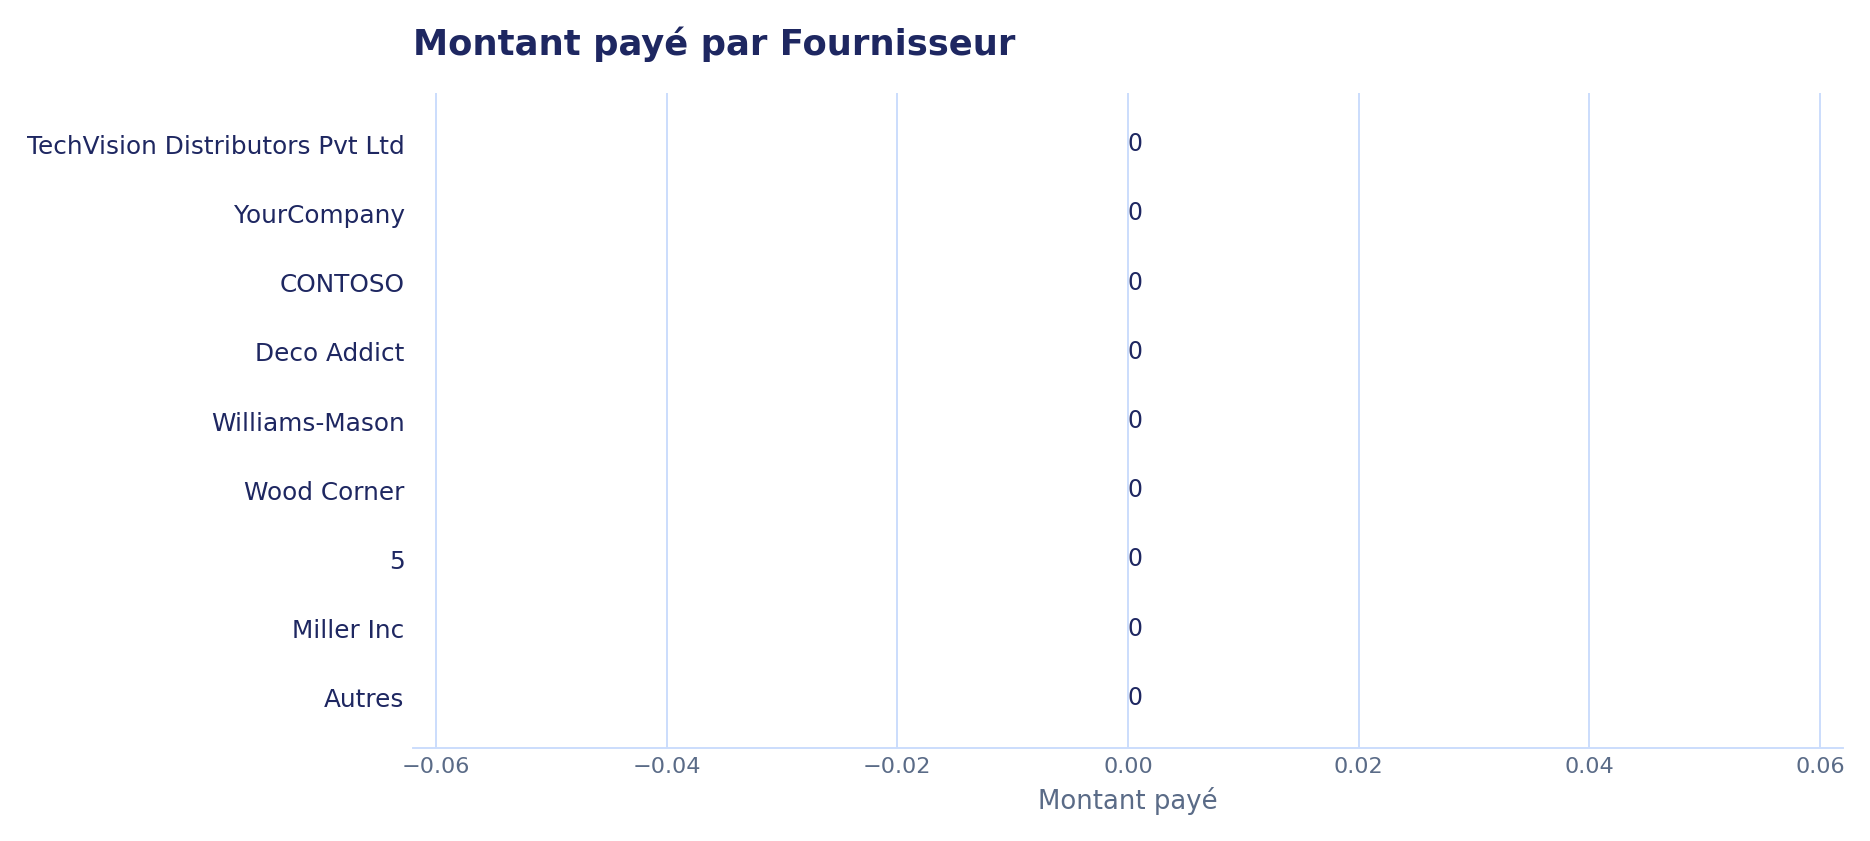
\includegraphics[width=0.85\textwidth]{images/graphique.png}
\caption[Graphique de synthese]{Graphique horizontal genere avec regroupement des categories principales.}
\label{fig:graphique}
\end{figure}

\section{Tracabilite}

Les rapports sont organises par timestamp. Cette organisation facilite la comparaison entre plusieurs executions et evite d'ecraser les resultats precedents.

\begin{figure}[H]
\center
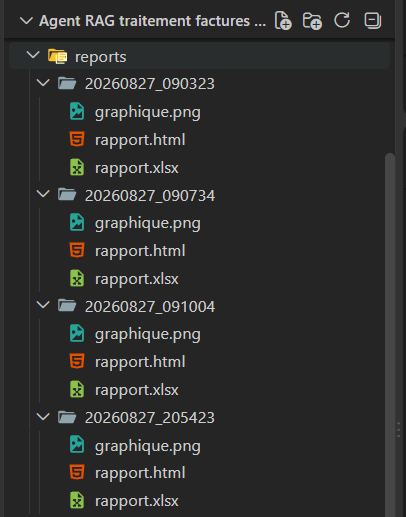
\includegraphics[width=0.9\textwidth]{images/organisation_par_timestamp.png}
\caption[Organisation par timestamp]{Organisation des sorties de reporting dans des dossiers horodates.}
\label{fig:timestamp}
\end{figure}

\begin{figure}[H]
\center
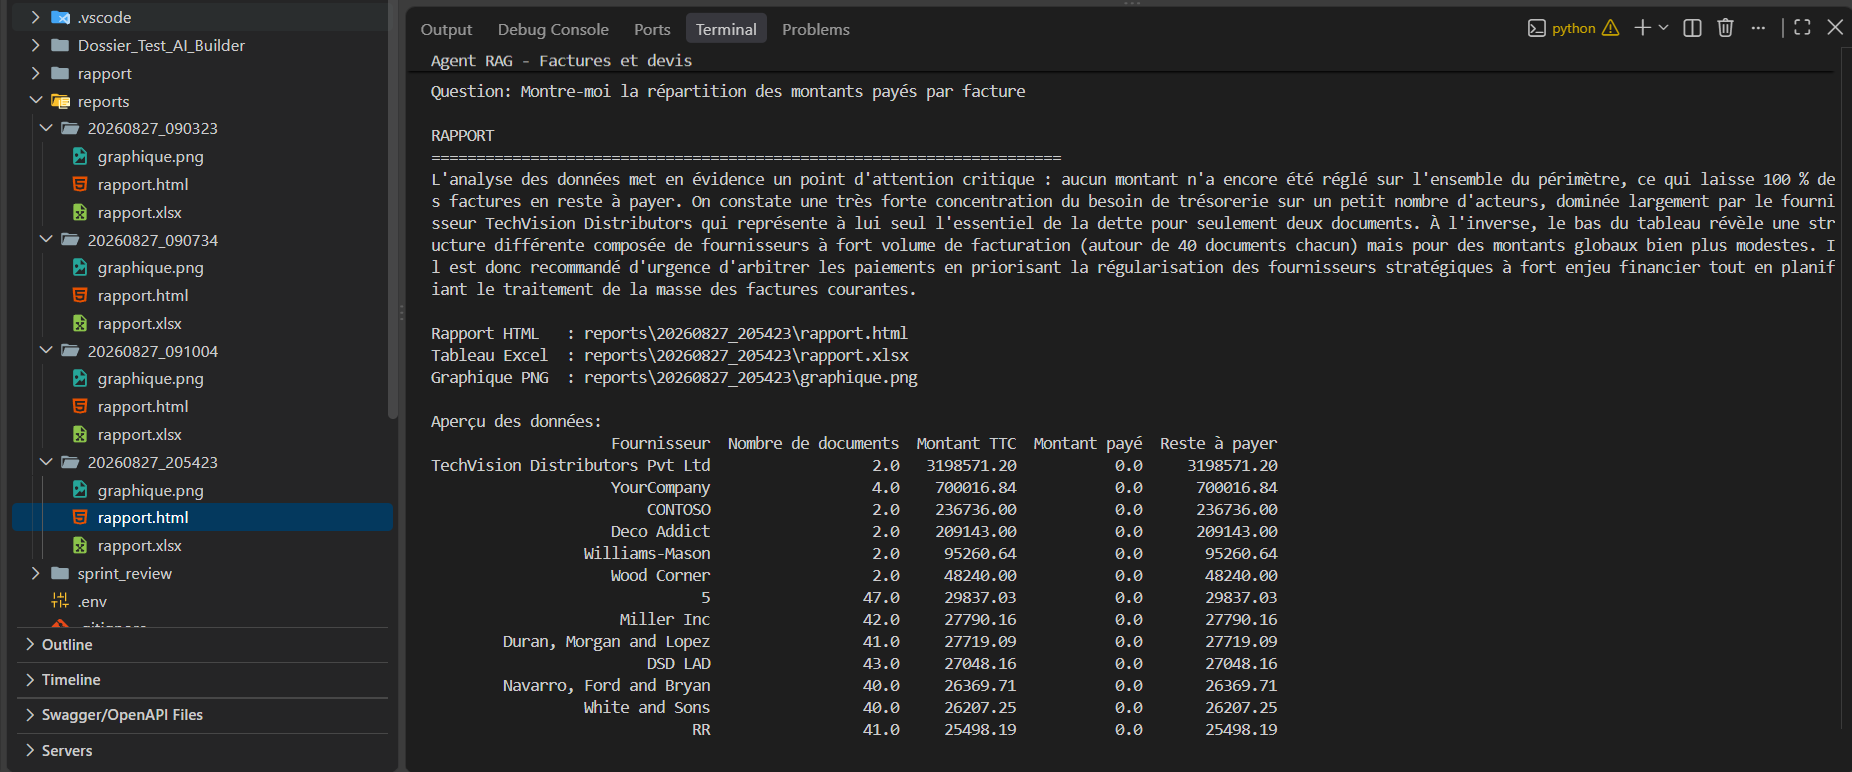
\includegraphics[width=0.9\textwidth]{images/rapport4.png}
\caption[Rapport final]{Exemple supplementaire de rapport genere par l'agent.}
\label{fig:rapport4}
\end{figure}

\section{Evaluation globale}

Le projet atteint les objectifs principaux: extraction de donnees, stockage structure, suivi des erreurs, embeddings, recherche hybride, reponses groundees et reporting automatique. Les tests ont egalement revele des points d'attention importants, notamment les quotas LLM, la stabilite des connexions longues et les differences de types entre les outils.
